\documentclass[12pt,letterpaper]{article}

\usepackage[spanish, es-tabla, es-nodecimaldot]{babel}
\usepackage[utf8x]{inputenc}
\usepackage{amsmath}

\usepackage{hyperref}
\usepackage{url}
\usepackage{textcomp}
\usepackage{gensymb}
\usepackage[dvipsnames]{xcolor}

\usepackage{parskip}
\usepackage{fancyhdr}
\usepackage{multicol}
\usepackage{vmargin}
\usepackage{setspace}
\usepackage{geometry}

\usepackage{float}
\usepackage{array}
\usepackage{graphicx}
\graphicspath{{Images/}}
\usepackage{wrapfig}
\usepackage{caption}
\usepackage{subcaption}

\setmarginsrb{2.0cm}{1.0cm}{2.0cm}{2.5cm}{0.5cm}{1cm}{1 cm}{1 cm} %{izq}{up}{der}{down}{Encabezado}

\pagestyle{fancy}
\fancyhf{}
\rhead{Lic. Física}
%\lhead{\thesection}
\cfoot{\thepage}


\title{ Comentarios, Desarrollos u Observaciones  }

\begin{document}


\begin{titlepage}
	\centering
    \vspace*{2cm}
	{\Huge Comentarios, Desarrollos u Observaciones \par}
	\vfill
	{\Large Desarrollo Experimental II \par}
	\vfill
	{\large\ Docente: Dra. Laura Lorenia Yeomans Reyna \par}
    \vfill
    {\large\ \textbf{Portafolio II}:\\ Simulación de Monte Carlo \par}
    \vfill
    {\large\ Martín Alejandro Paredes Sosa \par}
	\vfill
	% Bottom of the page
	{\large Semestre: 2018-1\par}
\end{titlepage}
\section*{Tarea III: Ejercicios para movimientos arbitrarios de partículas, condiciones periódicas y energía de la configuración }
A continuacion se muestran los cometarios y avances relacionados con la tarea 3 del portafolio II.
\vspace{-0.5cm}

\subsection*{Actividad 1: Sin Condiciones Periódicas}
La actividad consistio en realizar el movimiento de particulas de manera aleatoria, sin considerar condiciones periodicas, es decir la particulas no vuelven a entrar a la celda. 
	\begin{figure}[H]
		\centering

		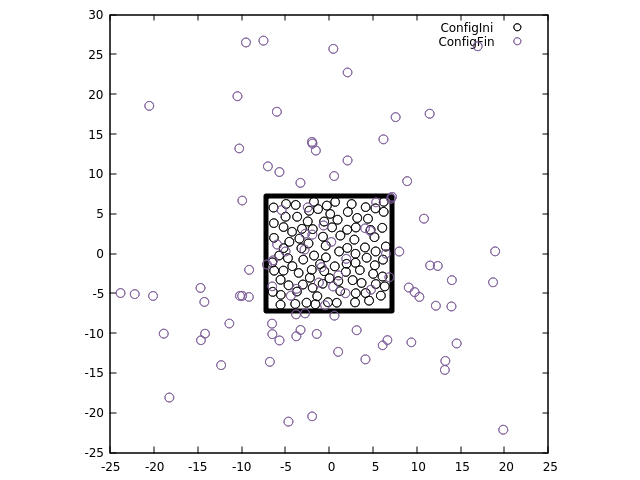
\includegraphics[scale=0.75]{Config_INI_FIN_2.png}
		\caption{Configuración Inicial con $n^*=0.5093$, con un $NStep=1000$ y un $\delta_{MAX}=0.5\sigma$}
	\end{figure}
	Se observa que las particulas se alejan consideradamente de las fronteras de la celda original.

\subsection*{Actividad 2}
La actividad consistio en realizar el movimiento de particulas de manera aleatoria, ahora considerando condiciones periodicas, es decir la particulas vuelven a entrar a la celda, cuando una sale, asi asegunrando que la concentración en la celda original se mantiene.
\begin{figure}[H]
		\centering
		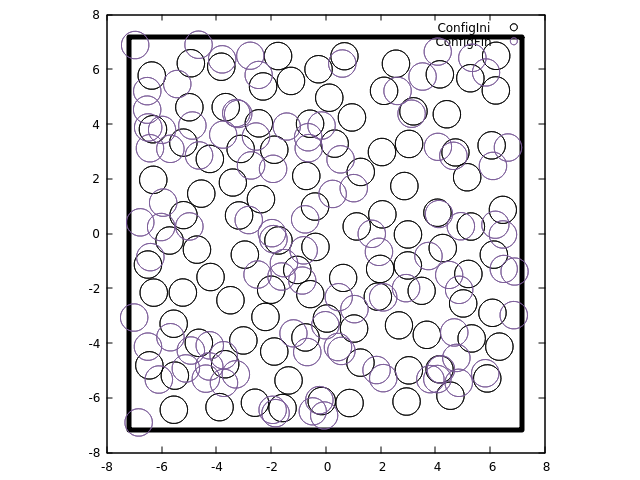
\includegraphics[scale=0.75]{Config_INI_FIN}
		\caption{Configuración Inicial con $n^*=0.5093$, con un $NStep=1000$ y un $\delta_{MAX}=0.5\sigma$}
	\end{figure}
Se observa que todas las particulas estan dentro de la celda original, ligeramente afuera pero sus centros siguen dentro de las fronteras. 

Estas dos actividades permiten observar la forma en la que se mueven las partículas. La aplicacion de condiciones periódicas es sencillo de implementar ya que consiste en volver a ingresar una partícula de lado opuesto de donde salio la otra.
\subsection*{Actividad 3}
La tercera actividad cosnsistia en seguir el movimiento de dos partículas aleatorias. Esto permite observar las condiciones periódicas en acción.

	\begin{figure}[H]
		\centering
		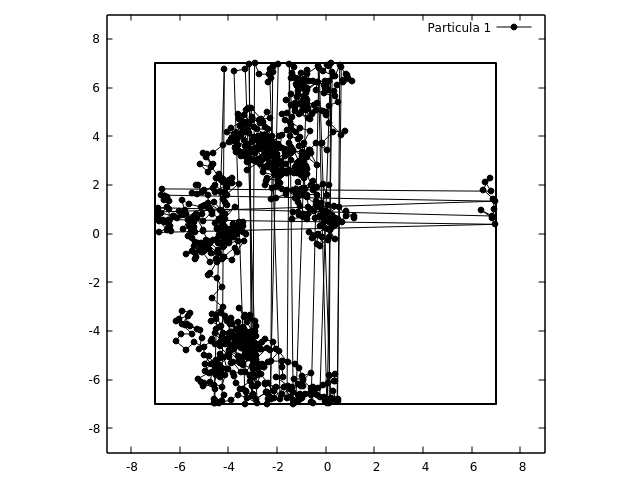
\includegraphics[width=0.49\linewidth]{Particula1.png}
		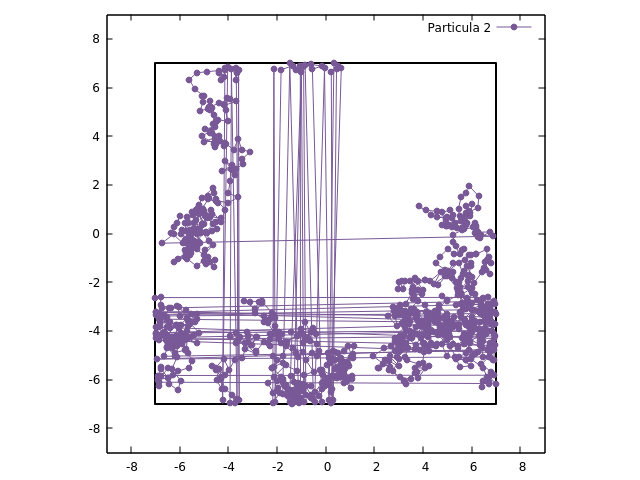
\includegraphics[width=0.49\linewidth]{Particula2.png}\\
		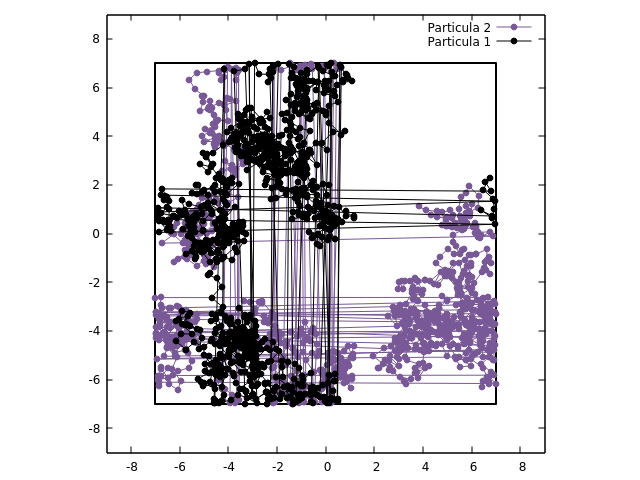
\includegraphics[width=0.75\linewidth]{Traza.png}
		\caption{ Con $n^*=0.5093$, con un $NStep=1000$ y un $\delta_{MAX}=0.5\sigma$. Se realizo la traza de las partículas 84 y 57.}
	\end{figure}
Se aprecia como cuando una particula sale de las fronteras de la celda esta entra de lado opuesto cuando aparecen las lineas largas que atraviesan la celda.

\subsection*{Actividad 4}
La cuarta actividad consistió en realizar lo mismo que las actividades anteriores solo que adapatando a tres dimensiones.
	\begin{figure}[H]
		\centering
		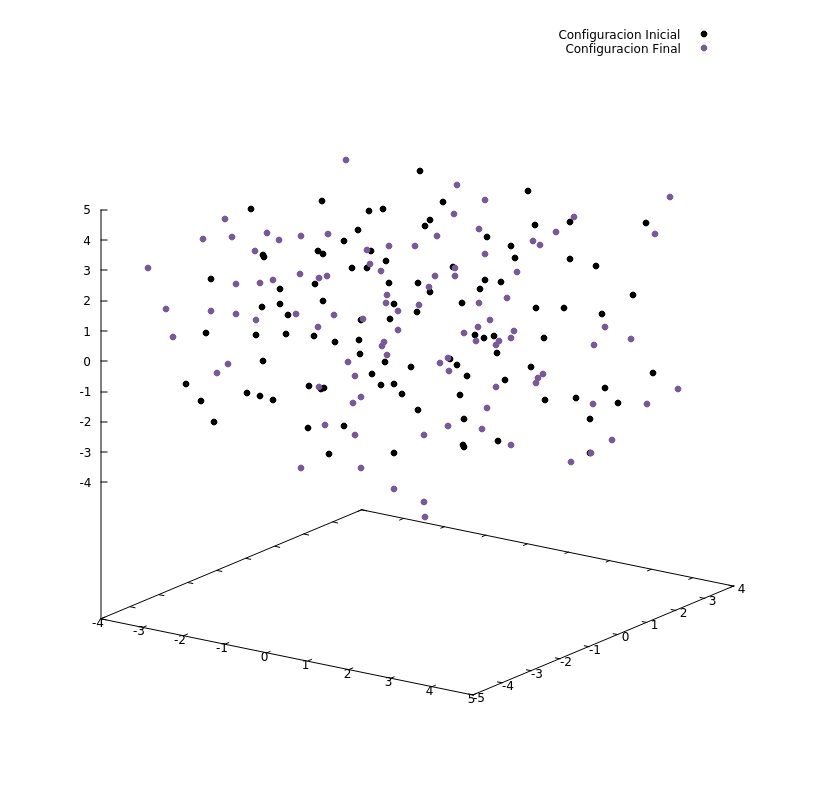
\includegraphics[width=0.5\linewidth]{ConfigS3D.png}
		\caption{ Con $n^*=0.1910$, con un $NStep=100000$ y un $\delta_{MAX}=0.5\sigma$.}
	\end{figure}
	\begin{figure}[H]
		\centering
		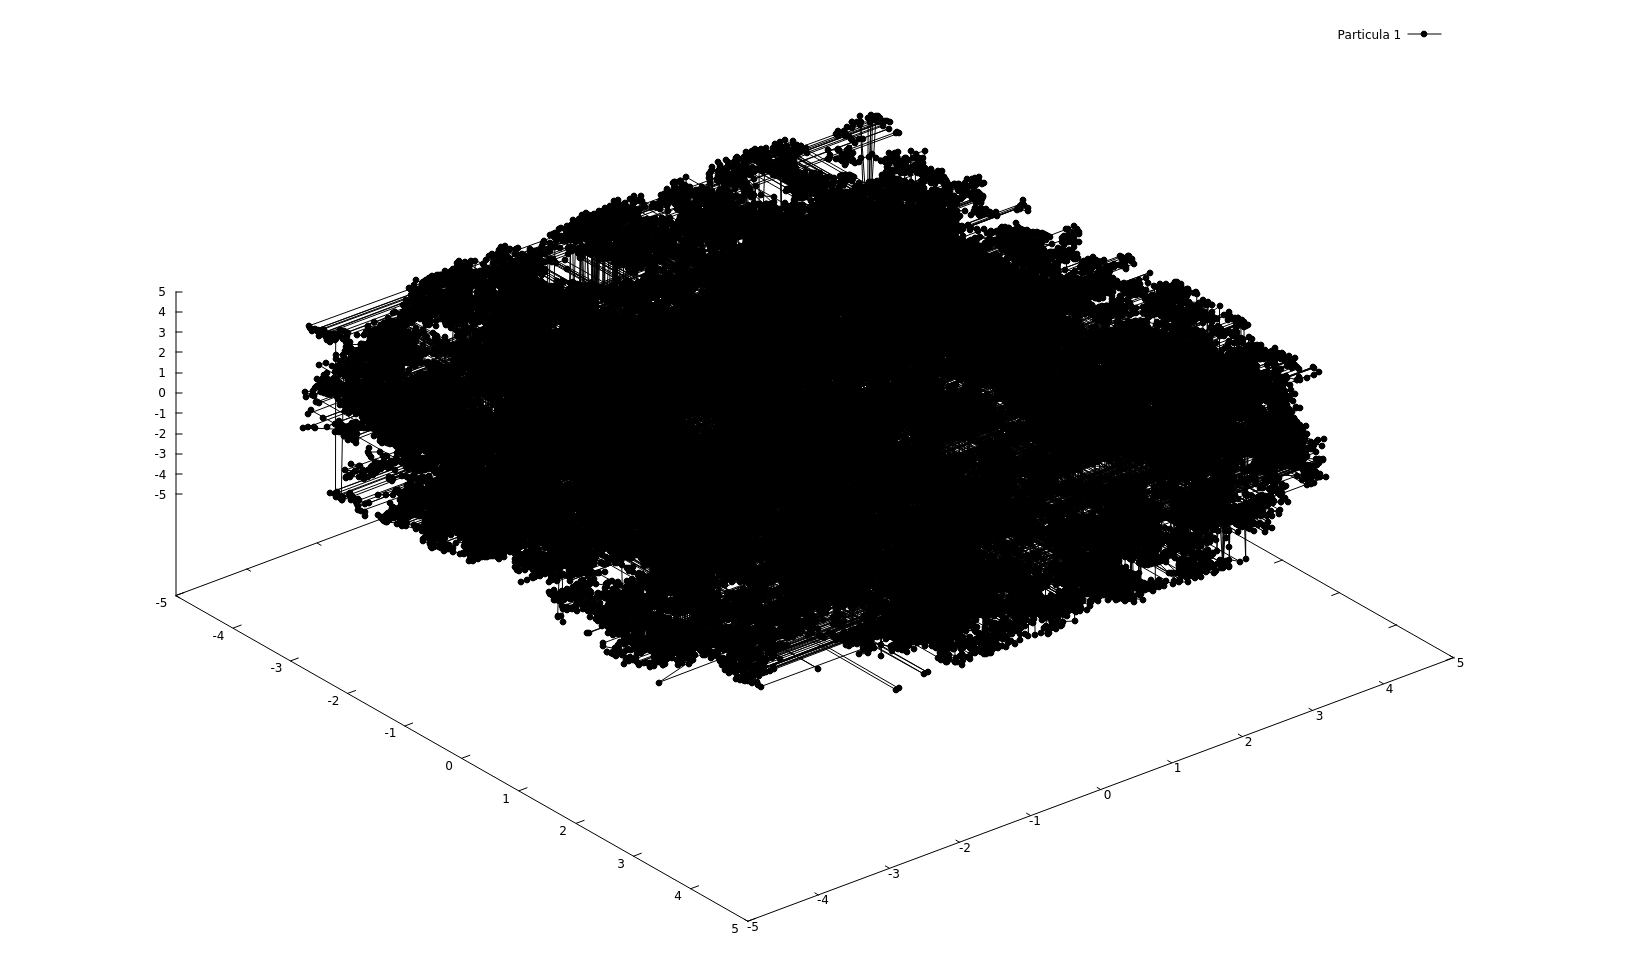
\includegraphics[width=0.49\linewidth]{Part1.png}
		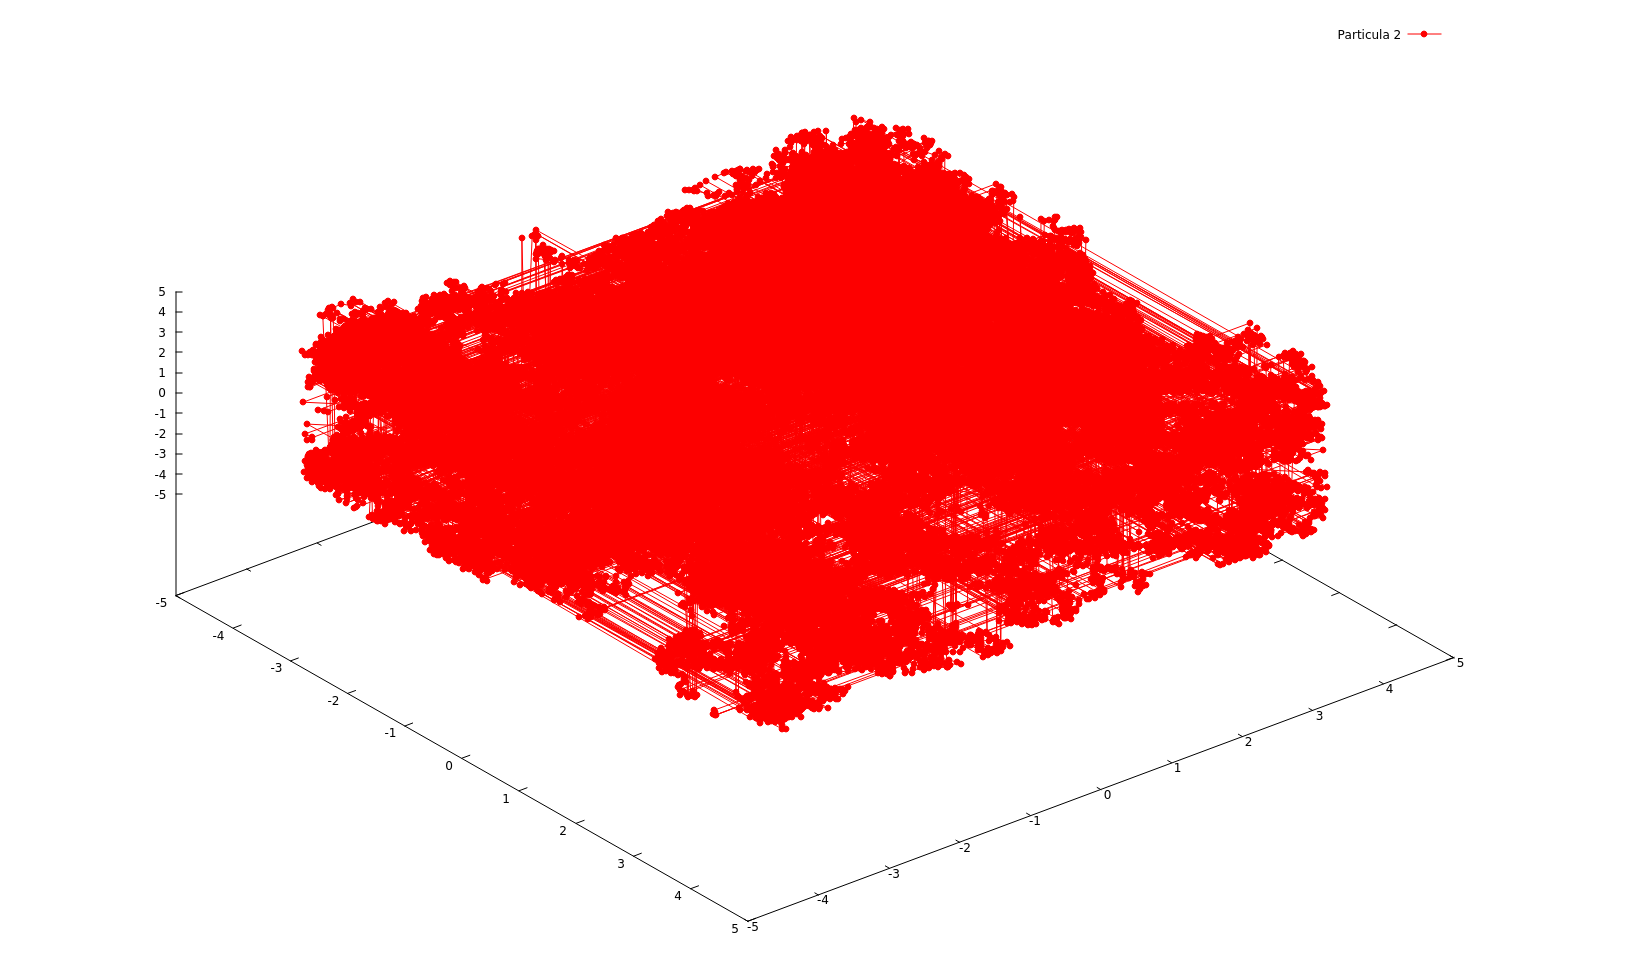
\includegraphics[width=0.49\linewidth]{Part2.png}
		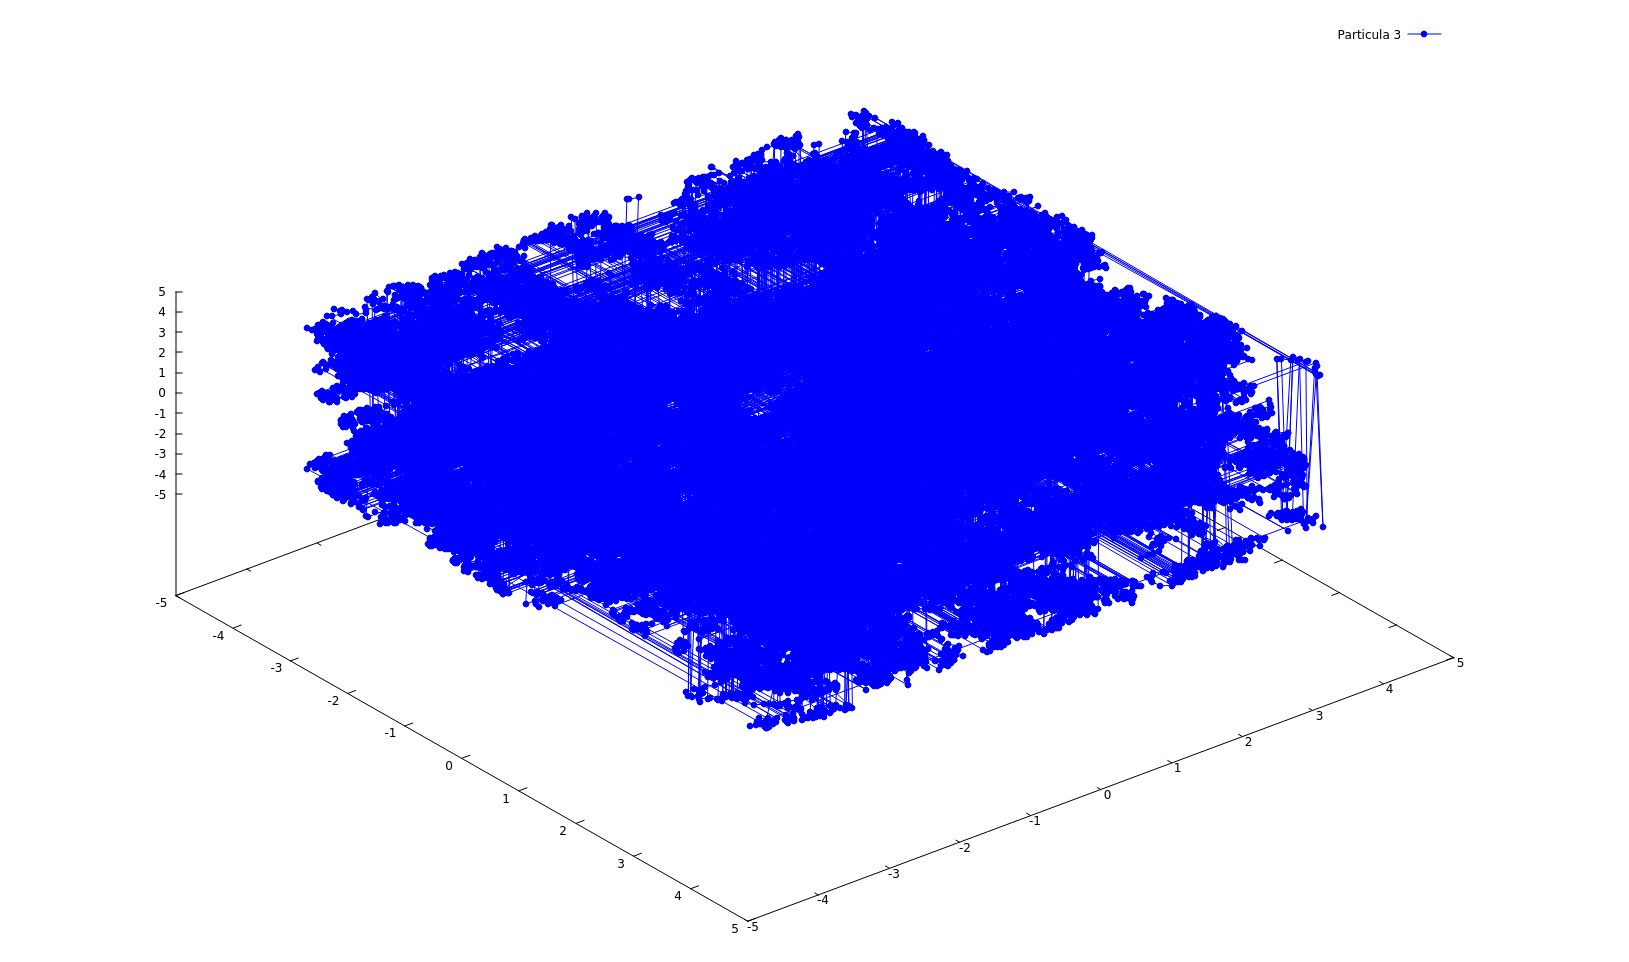
\includegraphics[width=0.49\linewidth]{Part3.png}
		\caption{Con $n^*=0.1910$, con un $NStep=100000$ y un $\delta_{MAX}=0.5\sigma$. Se realizo la traza de las partículas 84, 57 y 4.}
	\end{figure}
Se observa las configuraciones inicial y final de un arreglo en 3D. Las trazas de las partículas se aprecia algo parecido a la de la actividad 3 por las condiciones periódicas.

\subsection*{Actividad 5}
	\begin{figure}[H]
		\centering
		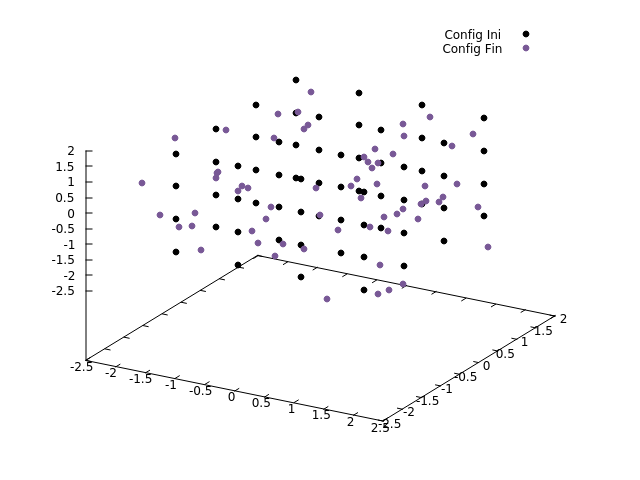
\includegraphics[width=0.5\linewidth]{ConfigS.png}
		\caption{ Con $n^*=1.0$, con un $NStep=1000$ y un $\delta_{MAX}=0.5\sigma$.}
	\end{figure}
	\begin{figure}[H]
		\centering
		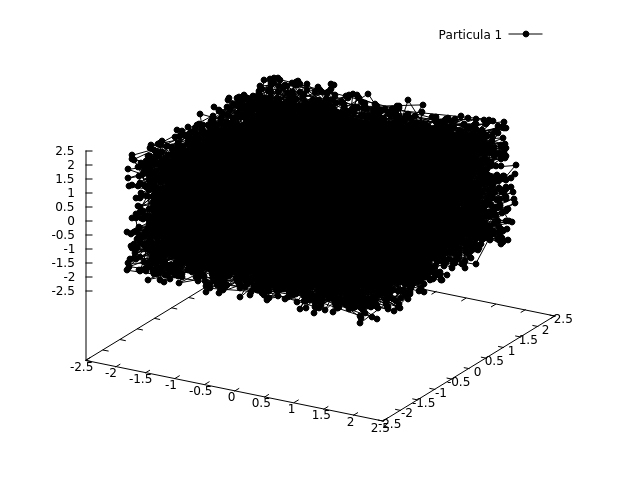
\includegraphics[width=0.49\linewidth]{Parti1.png}
		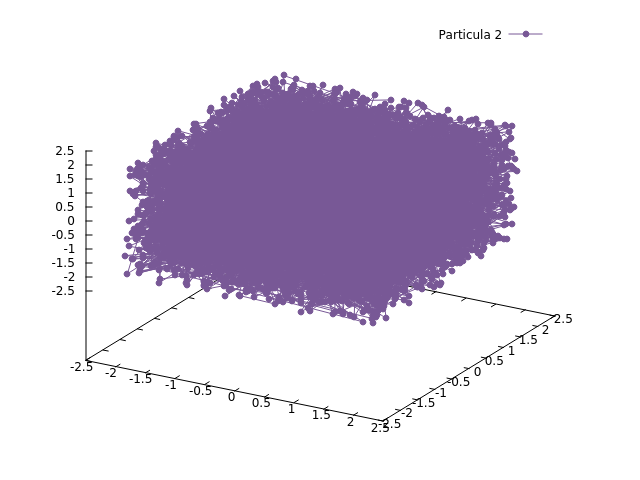
\includegraphics[width=0.49\linewidth]{Parti2.png}
		\caption{Con $n^*=1.0$, con un $NStep=1000$ y un $\delta_{MAX}=0.5\sigma$. Se realizo la traza de las partículas 64 y 36.}
	\end{figure}
	
	En la actividad se utilizó una configuración regular cúbica  en lugar de una aleatoria. y se observan las mismas cosas.
	
	\subsection*{Actividad 6}
	En esta actividad se realizo el cálculo de la energía de un sistema de disco duros (HD). Se obtuvo lo siguinte.
	\begin{figure}[H]
		\centering
		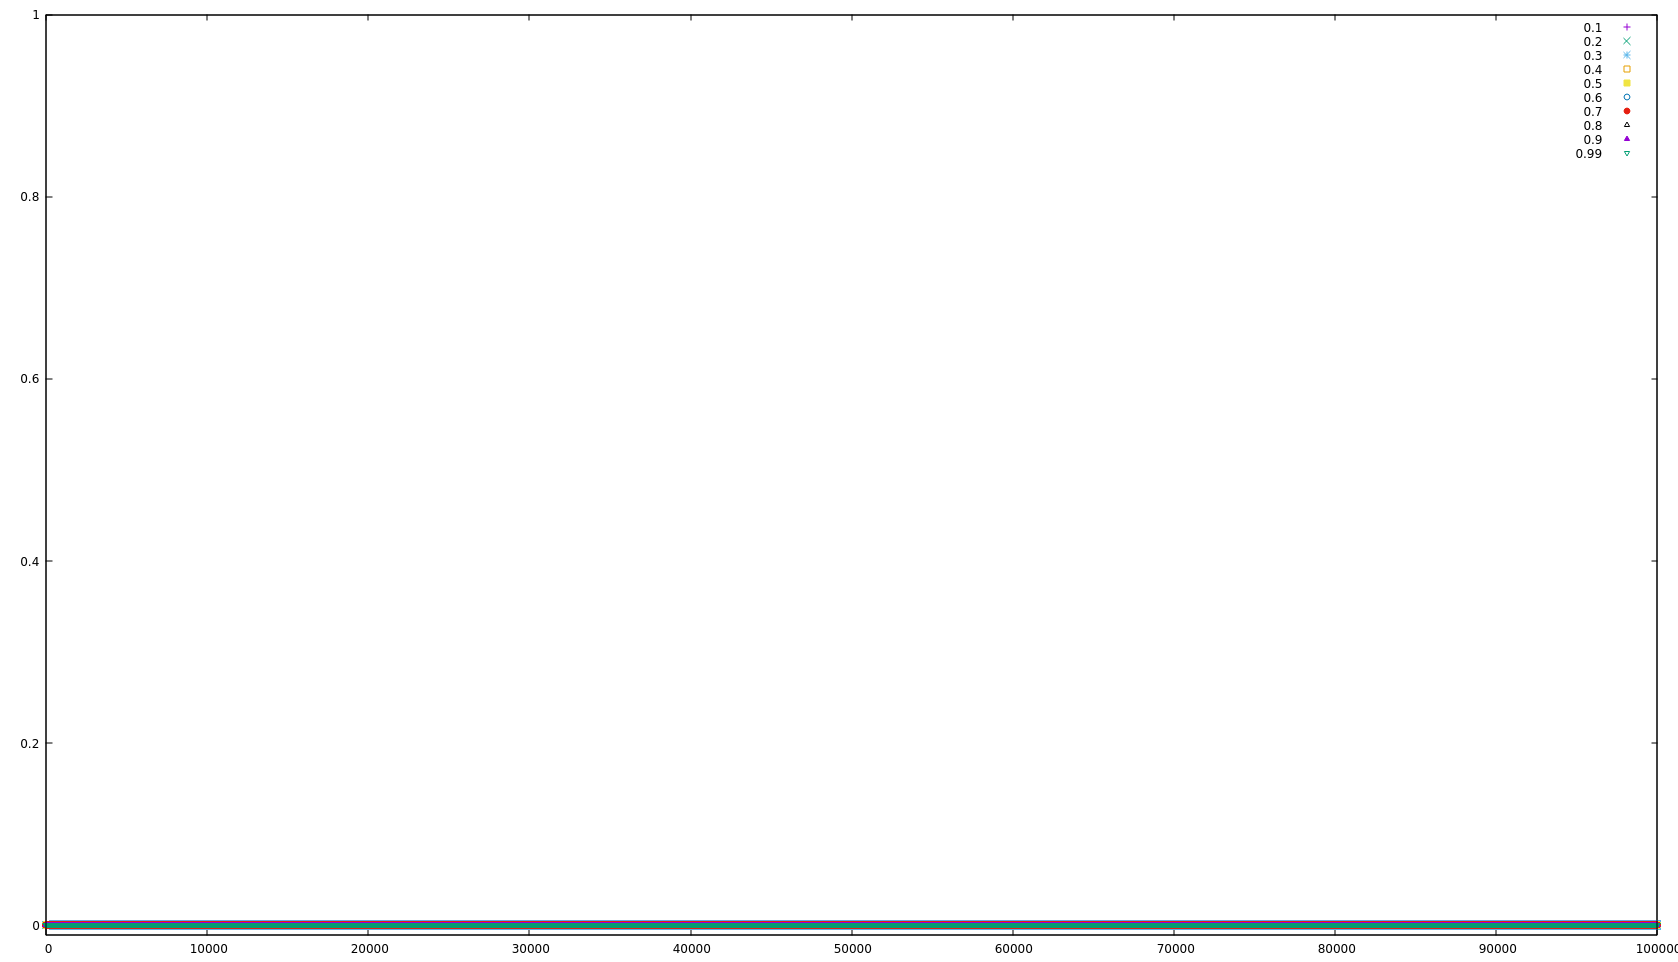
\includegraphics[width = 0.75\linewidth]{Terma.png}
		\caption{Termalizacion de HD para concentraciones de 0.1 a 0.99}
	\end{figure}
	Como es el potencial de discos duro, todas las configuraciones tuvieron energia 0 como era de esperarse.
\pagebreak
\section*{Tarea IV}
La tarea 4 consiste de una actividad, en la cual se implementó el código de montecarlo.
\subsection*{Actividad 7}














\end{document}

